%%%%%%%%%%%%%%%%%%%%%%%%%%%%%%%%%%%%%%%%%%%%%%%%%%%%%%%%%%%%%%%%%%%%%%%%%%%

\documentclass[a4paper,oneside,12pt]{article}
\usepackage{mystyle}

\begin{document}

\title{\Large\bf Real numbers}
\author{%%
  Minh Van Nguyen \\
  \url{mvngu@gmx.com}
}
\date{\today}
\maketitle

%%%%%%%%%%%%%%%%%%%%%%%%%%%%%%%%%%%%%%%%%%%%%%%%%%%%%%%%%%%%%%%%%%%%%%%%%%%

\section{Rational numbers}

A \emph{rational} number is a ratio of two integers.  A
rational number is also known as a fraction.  These are rational
numbers: $1/2$, $3/4$, $11/9$, and $-10/2$.  You write $5/2 \in \QQ$
to mean that $5/2$ belongs to the set of rational numbers.  The set of
all rational numbers is written as
\[
\QQ
=
\setdes{
  \frac{a}{b}
}{
  \pair{a}{b} \in \ZZ
  \text{ and }
  b \neq 0
}.
\]
This means that the set of rational numbers consists of all numbers of
the form $a/b$ such that $a$ and $b$ are integers, but $b$ cannot be
zero.  The top integer $a$ is called the \emph{numerator} and the
bottom integer $b$ is called the \emph{denominator}.  If $b = 1$, then
$a/b = a/1 = a$ and consequently any integer is also a rational
number.

\begin{exercise}
Provide an example of a rational number that is also an integer.  Why
is your number an integer?
\end{exercise}

\ifbool{showSolution}{
\begin{solution}
The rational number $2/1$ is also an integer because it can be written
as $2/1 = 2$ and $2$ is an integer.
\end{solution}
}{}

\begin{exercise}
Give an example of a rational number that is not an integer.  Explain
why your number is not an integer.
\end{exercise}

\ifbool{showSolution}{
\begin{solution}
The ratio $1/2$ is not an integer because $1/2$ cannot be simplified
to any integer.
\end{solution}
}{}

\begin{exercise}
If $a/b$ is a rational number, why must you have $b \neq 0$?  Consider
the examples of $1/4$ and $1/0$.
\end{exercise}

\ifbool{showSolution}{
\begin{solution}
If in the rational number $a/b$ you have $b = 0$, then the ratio
$a / 0$ is not defined.  This means that as $b$ comes closer and
closer to zero, the value of the ratio $a/b$ does not come to a fixed
number.
\end{solution}
}{}

If $a/b$ is a rational number, there are many rational numbers that
have the same value as $a/b$.  For example, the ratio $1/2$ is the
same as the ratios $2/4$, $3/6$, and $4/8$.  The reason is that you
can write
%%
\begin{align*}
\frac{1}{2}
&=
\frac{1}{2} \times \frac{2}{2} \\[4pt]
&=
\frac{1}{2} \times \frac{3}{3} \\[4pt]
&=
\frac{1}{2} \times \frac{4}{4}.
\end{align*}
%%
In fact, if $c$ is any integer such that $c \neq 0$, then
\[
\frac{a}{b}
=
\frac{a}{b} \times \frac{c}{c}
=
\frac{ac}{bc}
\]
where the ratio $c/c$ can be simplified as $c/c = 1$.  The set $\ZZ$
of integers has an infinite number of elements because the sequence
$\seqi{1}{2}{3}$ of positive integers gets bigger and bigger and goes
on forever.  Furthermore, the sequence $\seqi{-1}{-2}{-3}$ of negative
integers gets smaller and smaller and also goes on forever.  In other
words, if $a/b$ is a rational number, then it is easy find an infinite
number of rational numbers that have the same value as $a/b$.  The
above is summarised as:

\begin{theorem}
\label{thm:infinitely_many_rationals_same_value}
If $a/b$ is a rational number such that $b \neq 0$, then there are
infinitely many rational numbers that have the same value as $a/b$.
\end{theorem}

It is because of \Theorem{thm:infinitely_many_rationals_same_value}
that you can simplify a fraction.  If a rational number $a/b$ can be
simplified, then there must be a rational number $c/d$ that has the
same value as $a/b$ but the numerator
$\absoluteValue{c} < \absoluteValue{a}$ and the denominator
$\absoluteValue{d} < \absoluteValue{b}$.  The expression
$\absoluteValue{x}$ is defined below.

\begin{definition}
\textbf{Absolute value.}
Given any number $x$, the expression $\absoluteValue{x}$ is called the
\emph{absolute value} of $x$ and is defined as
%%
\begin{equation}
\label{eqn:define_absolute_value}
\absoluteValue{x}
=
\begin{cases}
x,  & \text{if $x \geq 0$}, \\[4pt]
-x, & \text{otherwise}.
\end{cases}
\end{equation}
\end{definition}

For example, the absolute value of $0$ is $0$, the absolute value of
$3$ is $3$, and the absolute value of any positive number $y$ is $y$
itself.  You obtain the absolute value of a negative number by
multiplying the number by $-1$.  For example, the absolute value of
$-7$ is $\absoluteValue{-7} = -1 \times (-7) = 7$.

\begin{exercise}
Simplify the expression $\frac{1}{4} + \frac{1}{2}$.
\end{exercise}

\ifbool{showSolution}{
\begin{solution}
The expression $\frac{1}{4} + \frac{1}{2}$ can be simplified as
follows:
%%
\begin{align*}
\frac{1}{4} + \frac{1}{2}
&=
\frac{1}{4}
+
\frac{1}{2} \times \frac{2}{2} \\[4pt]
&=
\frac{1}{4}
+
\frac{2}{4} \\[4pt]
&=
\frac{3}{4}.
\end{align*}
\end{solution}
}{}

\begin{exercise}
Can the rational number $15 / 21$ be simplified any further?  If yes,
provide a simplified version of $15 / 21$.  If no, explain why not.
\end{exercise}

\ifbool{showSolution}{
\begin{solution}
The numerator $15$ and the denominator $21$ both have $3$ as a common
factor.  Then the rational number $15 / 21$ can be simplified as:
%%
\begin{align*}
\frac{15}{21}
&=
\frac{
  3 \times 5
}{
  3 \times 7
} \\[4pt]
&=
\frac{5}{7}.
\end{align*}
\end{solution}
}{}

\begin{exercise}
Simplify the fraction $-28 / 35$ as much as possible.
\end{exercise}

\ifbool{showSolution}{
\begin{solution}
The numerator and denominator both have $7$ as a common factor so the
fraction $-28 / 35$ can be simplified as:
%%
\begin{align*}
-\frac{28}{35}
&=
-\frac{
  7 \times 4
}{
  7 \times 5
} \\[4pt]
&=
-\frac{4}{5}.
\end{align*}
%%
Note that $\absoluteValue{-4} = 4$ and $\absoluteValue{-28} = 28$ and
so $\absoluteValue{-4} < \absoluteValue{-28}$ even though
$-28 < -4$.
\end{solution}
}{}

\begin{exercise}
Explain why the rational number $3/7$ cannot be simplified any
further.
\end{exercise}

\ifbool{showSolution}{
\begin{solution}
The only factor that $3$ and $7$ have in common is $1$.  Therefore the
rational number $3/7$ cannot be simplified any further.
\end{solution}
}{}


%%%%%%%%%%%%%%%%%%%%%%%%%%%%%%%%%%%%%%%%%%%%%%%%%%%%%%%%%%%%%%%%%%%%%%%%%%%

\section{Irrational numbers}

An \emph{irrational} number is any number that cannot be written as a
ratio $a / b$, where $a$ and $b$ are integers with $b \neq 0$.  The
number $\sqrt{2}$ is an irrational number so it cannot be an integer
and cannot be written as a ratio of two integers.  But how did you
know that $\sqrt{2}$ is irrational?  How would you prove that
$\sqrt{2}$ is irrational?  The fact that $\sqrt{2}$ is irrational can
be demonstrated by using a technique called
\emph{proof by contradiction}, which is a method of indirect
reasoning.  The general idea of proof by contradiction is as follows.
Any statement is either true or false.  To prove that a statement $S$
is false, you assume that it is true and then work out a contradiction
that results from assuming the truth of $S$.  Since the truth of the
statement $S$ has led to a contradiction, it must be that $S$ is
false.  Before proving that $\sqrt{2}$ is irrational, let's practice
using the technique of proof by contradiction.

Let $a$ be an integer.  You already know that if $a$ is even, then the
product $a^2 = a \times a$ is also even.  What about going backward?
If $a^2$ is even, is it true that $a$ is also even?  You can show that
the last statement is true via proof by contradiction.

\begin{theorem}
\label{thm:a_squared_even_implies_a_even}
Let $a$ be an integer.  If $a^2$ is even, then $a$ is even.
\end{theorem}

\begin{proof}
The statement of the theorem tells you that $a^2$ is even so you can
assume that $a^2$ is even.  Use the definition of even integers to
write $a^2$ as $a^2 = 2k$, where $k$ is some other integer.  There are
two possibilities for the integer $a$.  Either $a$ is even or it is
odd.  To derive a contradiction, assume that $a$ is odd.  Use the
definition of odd integers to write $a$ as $a = 2r + 1$, where $r$ is
another integer.  You know that the product of two odd integers is
also an odd integer.  Use this result to see that $a^2 = (2r + 1)^2$
is odd.  However, you assumed above that $a^2$ is even.  You have a
contradiction because $a^2$ cannot be both even and odd.  The
contradiction arises becauase you assumed that $a$ is odd.  Therefore
you conclude that $a$ is even.
\end{proof}

\begin{theorem}
The number $\sqrt{2}$ is irrational.
\end{theorem}

\begin{proof}
The number $\sqrt{2}$ is either rational or irrational.  To derive a
contradiction, assume that $\sqrt{2}$ is rational.  Since $\sqrt{2}$
is rational, it can be written as a ratio
%%
\begin{equation}
\label{eqn:root_2_as_ratio}
\sqrt{2}
=
\frac{a}{b}
\end{equation}
%%
where $a$ and $b$ are positive integers with $b \neq 0$.  You may
assume that the ratio $a / b$ cannot be simplified any further.  (If
$a/b$ can be simplified, you simplify the ratio as much as possible
until you cannot simplify any more.)  Square both sides of
\Equation{eqn:root_2_as_ratio} and you can write
\Equation{eqn:root_2_as_ratio} as
\[
(\sqrt{2})^2
=
\parenthesis*{
  \frac{a}{b}
}^2
\]
which simplifies to $2 = a^2 / b^2$.  Now solve for $a^2$ to see that
\Equation{eqn:root_2_as_ratio} can also be written as
%%
\begin{equation}
\label{eqn:root_2_a_square_is_even}
2b^2
=
a^2.
\end{equation}
%%
In other words, $a^2$ is even and you may conclude by
\Theorem{thm:a_squared_even_implies_a_even} that $a$ must be even as
well.  Use the definition of even integers to write $a$ as $a = 2k$,
where $k$ is some other integer.  Substitute $a = 2k$ into
\Equation{eqn:root_2_a_square_is_even} and you get $2b^2 = (2k)^2$.
Simplify the latter equation and you see that
\Equation{eqn:root_2_as_ratio} can also be written as
%%
\begin{equation}
\label{eqn:root_2_b_square_is_even}
b^2
=
2k^2.
\end{equation}
%%
Equation~\eqref{eqn:root_2_b_square_is_even} says that $b^2$ is even.
You may conclude by \Theorem{thm:a_squared_even_implies_a_even} that
$b$ is also even.  What you now have is that both $a$ and $b$ are
even and so the ratio $a / b$ can be simplified by dividing each of
the numerator and denominator by $2$.  You have a contradiction
because you assumed above that $a / b$ cannot be simplified any
further.  The contradiction comes about because you assumed that
$\sqrt{2}$ is a rational number.  Therefore you may conclude that
$\sqrt{2}$ is irrational.
\end{proof}

\begin{exercise}
Is the number $(\sqrt{2})^2$ rational or irrational?  If yes, explain
why.  If no, explain why not.
\end{exercise}

\ifbool{showSolution}{
\begin{solution}
Since the number $(\sqrt{2})^2$ is positive, it can be written as
%%
\begin{align*}
(\sqrt{2})^2
&=
(2^{1/2})^2 \\[4pt]
&=
2^{2/2} \\[4pt]
&=
2.
\end{align*}
%%
Then $(\sqrt{2})^2 = 2$ is an integer and therefore a rational number
because you can write $2 = 2/1$.
\end{solution}
}{}

\begin{exercise}
Is the number $(\sqrt{2})^4$ rational or irrational?
\end{exercise}

\ifbool{showSolution}{
\begin{solution}
The number $(\sqrt{2})^4$ can be written as
%%
\begin{align*}
(\sqrt{2})^4
&=
(\sqrt{2})^2 \times (\sqrt{2})^2 \\[4pt]
&=
2^2 \\[4pt]
&=
4.
\end{align*}
%%
Therefore $(\sqrt{2})^4$ is a rational number.
\end{solution}
}{}

\begin{exercise}
Is the number $(\sqrt{2})^6$ rational or irrational?
\end{exercise}

\ifbool{showSolution}{
\begin{solution}
The number $(\sqrt{2})^6$ can be written as
%%
\begin{align*}
(\sqrt{2})^6
&=
(\sqrt{2})^2 \times (\sqrt{2})^2 \times (\sqrt{2})^2 \\[4pt]
&=
2^3 \\[4pt]
&=
8.
\end{align*}
%%
Therefore $(\sqrt{2})^6$ is a rational number.
\end{solution}
}{}


%%%%%%%%%%%%%%%%%%%%%%%%%%%%%%%%%%%%%%%%%%%%%%%%%%%%%%%%%%%%%%%%%%%%%%%%%%%

\section{Real numbers}

The set of \emph{real} numbers is made up of all rational and all
irrational numbers.  The set of real numbers is written as $\RR$.  For
example, the ratio $3/7$ is a real number, the square root $\sqrt{2}$
is a real number, and the integer $42$ is a real number.  Given any
number $x \in \RR$, you now have the following situation.  The number
$x$ is either rational or irrational.  If $x$ is irrational, then it
cannot be written as a ratio of two integers.  On the other hand, if
$x$ is rational, then it can be written as $x = a / b$ with $a$ and
$b$ being integers such that $b \neq 0$.  It might happen that
$b = 1$, in which case $x$ would be an integer.  The above is
summarised in the number tree of \Figure{fig:number_tree}.

\begin{figure}[!htbp]
\centering
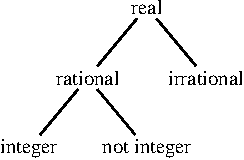
\includegraphics[scale=1.1]{image/02/number-tree.pdf}
\caption{%%
  The number tree shows the relationship among the different types of
  numbers.  The tree shows that a real number $x$ can be either
  rational or irrational.  If $x$ is rational, then it can be either
  an integer or not written as an integer.
}
\label{fig:number_tree}
\end{figure}

\begin{exercise}
Explain why any integer is a real number.
\end{exercise}

\ifbool{showSolution}{
\begin{solution}
Any integer is also a rational number.  Since a rational number is
also a real number, it follows that any integer is also a real
number.
\end{solution}
}{}

\begin{exercise}
How would you represent a real number as a picture?
\end{exercise}

\ifbool{showSolution}{
\begin{solution}
A real number can be represented as a point on the number line.
\end{solution}
}{}

\begin{exercise}
Simplify the expression
$\displaystyle{
  \frac{
    3 \times 2 + (11 - 5)
  }{
    2 \times (3 + 7)
  }
}$.
\end{exercise}

\ifbool{showSolution}{
\begin{solution}
The expression
$\displaystyle{
  \frac{
    3 \times 2 + (11 - 5)
  }{
    2 \times (3 + 7)
  }
}$
can be simplified as
%%
\begin{align*}
\frac{
  3 \times 2 + (11 - 5)
}{
  2 \times (3 + 7)
}
&=
\frac{
  3 \times 2 + 6
}{
  2 \times (3 + 7)
} \\[4pt]
&=
\frac{
  3 \times 2 + 6
}{
  2 \times 10
} \\[4pt]
&=
\frac{
  6 + 6
}{
  20
} \\[4pt]
&=
\frac{
  12
}{
  20
} \\[4pt]
&=
\frac{
  3
}{
  5
}.
\end{align*}
\end{solution}
}{}

\begin{exercise}
Simplify the expression
\[
E
=
\frac{
  3 m c^2
}{
  (6 - 4) + 1
}.
\]
\end{exercise}
\ifbool{showSolution}{
  \begin{solution}
  \begin{align*}
  E
  &=
  \frac{
    3 m c^2
  }{
    (6 - 4) + 1
  } \\[4pt]
  &=
  \frac{
    3 m c^2
  }{
    2 + 1
  } \\[4pt]
  &=
  \frac{
    3 m c^2
  }{
    3
  } \\[4pt]
  &=
  m c^2.
  \end{align*}
  \end{solution}
}{}

\begin{exercise}
Simplify the expression $(\frac{2}{4})^3$ in two different ways.
\end{exercise}

\ifbool{showSolution}{
\begin{solution}
One way is to first work out the powers and then simplify the
fraction:
%%
\begin{align*}
\parenthesis*{
  \frac{2}{4}
}^3
&=
\frac{2^3}{4^3} \\[4pt]
&=
\frac{
  2 \times 2 \times 2
}{
  4 \times 4 \times 4
} \\[4pt]
&=
\frac{8}{64} \\[4pt]
&=
\frac{1}{8}.
\end{align*}
%%
Another way is to first simplify the fraction and then work out the
powers:
%%
\begin{align*}
\parenthesis*{
  \frac{2}{4}
}^3
&=
\parenthesis*{
  \frac{1}{2}
}^3 \\[4pt]
&=
\frac{
  1 \times 1 \times 1
}{
  2 \times 2 \times 2
} \\[4pt]
&=
\frac{1}{8}.
\end{align*}
\end{solution}
}{}

\begin{exercise}
\label{ex:absolute_value_is_nonnegative}
If $x$ is any real number, explain why the absolute value
$\absoluteValue{x} \geq 0$.
\end{exercise}

\ifbool{showSolution}{
\begin{solution}
Since $x$ is any real number, you have two cases: either $x < 0$ or
$x \geq 0$.  First, assume that $x < 0$.  From
\Equation{eqn:define_absolute_value}, the absolute value
$\absoluteValue{x} = -1 \times x$.  Since $x < 0$, multiplying both
sides of the inequality by $-1$ reverses the inequality sign and
you obtain $-x > 0$.  This means that $\absoluteValue{x} > 0$.
Second, assume that $x \geq 0$.  Then
\Equation{eqn:define_absolute_value} also shows that
$\absoluteValue{x} \geq 0$.  Therefore you have
$\absoluteValue{x} \geq 0$ for any $x \in \RR$.
\end{solution}
}{}


\newpage
%%%%%%%%%%%%%%%%%%%%%%%%%%%%%%%%%%%%%%%%%%%%%%%%%%%%%%%%%%%%%%%%%%%%%%%%%%%

\section*{Problem}

\begin{problem}
\item Give an example of something that can be represented as a
  rational number.
\ifbool{showSolution}{
  \begin{solution}
  The number of oranges you have eaten divided by the number of
  oranges you have altogether.
  \end{solution}
}{}

\item Present an example of something that can be represented as an
  irrational number.
\ifbool{showSolution}{
  \begin{solution}
  The \emph{unit circle} is a circle whose radius is one unit; see
  \Figure{fig:unit_circle}.  If a circle has radius $r$, then its area
  can be calculated as $\pi r^2$.  Since the radius of the unit circle
  is $r = 1$, it follows that the unit circle has an area of
  $\pi r^2 = \pi \times 1^2 = \pi$.  Therefore the area of a unit
  circle can be represented as an irrational number, i.e.~the number
  $\pi$.
  %%
  \begin{figure}[!htbp]
  \centering
  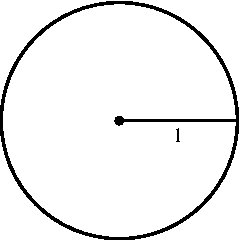
\includegraphics[scale=1]{image/02/unit-circle.pdf}
  \caption{%%
    The unit circle has a radius of one unit.  When you say
    ``one unit'' you do not care about the unit of measurement.  The
    length of the radius might be measured in terms of millimetre,
    centimetre, metre, or something else.  You are not concerned about
    these.  You only know that whatever standard of measurement is
    used, you want a value of one in terms of the scale of measurement
    that was used to measure the radius.  So the phrase ``one unit''
    can mean: one inch, one centimetre, one kilometre, etc.
  }
  \label{fig:unit_circle}
  \end{figure}
  \end{solution}
}{}

\item Provide an example of something that can be represented as a
  real number.
\ifbool{showSolution}{
  \begin{solution}
  The area of your house.
  \end{solution}
}{}

\item Explain what is wrong with the following expansion:
  %%
  \begin{equation}
  \label{eqn:wrong_expansion}
  \begin{aligned}
  -4 (3x - 2y)
  &=
  (-4)(3x) - 4(2y) \\[4pt]
  &=
  -12x - 8y.
  \end{aligned}
  \end{equation}
\ifbool{showSolution}{
  \begin{solution}
  Use the distributive laws to expand the expression $-4 (3x - 2y)$ as
  follows:
  %%
  \begin{align*}
  -4 (3x - 2y)
  &=
  (-4)(3x) - (-4)(2y) \\[4pt]
  &=
  -12x - (-8y) \\[4pt]
  &=
  -12x + 8y.
  \end{align*}
  %%
  The expansion~\eqref{eqn:wrong_expansion} is wrong.  The last term
  should be $+8y$, not $-8y$.
  \end{solution}
}{}

\item Let $x$ be a real number such that $x \neq 0$.  The expression
  $\absoluteValue{x} / x$ can take on two different values.  What are
  those two values?
\ifbool{showSolution}{
\begin{solution}
\Exercise{ex:absolute_value_is_nonnegative} shows that if
$y \in \RR$ then $\absoluteValue{y} \geq 0$.  Since $x \neq 0$, then
$\absoluteValue{x} > 0$.  In other words, the expression
$\absoluteValue{x} / x$ means that you have a positive number divided
by a number that can be either negative or positive.  If $x < 0$, then
$x = -\absoluteValue{x}$ and you have
$\frac{\absoluteValue{x}}{-\absoluteValue{x}} = -1$.  Otherwise
$x > 0$ and you have
$\frac{\absoluteValue{x}}{x} = \frac{x}{x} = 1$.  Therefore you have
\[
\frac{\absoluteValue{x}}{x}
=
\begin{cases}
-1, & \text{if $x < 0$}, \\[4pt]
1,  & \text{if $x > 0$}.
\end{cases}
\]
\end{solution}
}{}

\item Let $a$ and $b$ be integers such that $b \neq 0$.  Suppose the
  rational number $a/b$ cannot be simplified any further.  Can the
  ratio $6a / 12b$ be simplified any further?  If yes, provide a
  simplified version.  If no, explain why not.
\ifbool{showSolution}{
  \begin{solution}
  The integers $6$ and $12$ both have $6$ as a common factor.  Then
  you can simplify $\displaystyle{\frac{6a}{12b}}$ as
  %%
  \begin{align*}
  \frac{6a}{12b}
  &=
  \frac{
    6a
  }{
    6 \times 2b
  } \\[4pt]
  &=
  \frac{a}{2b}.
  \end{align*}
  \end{solution}
}{}

\item Suppose $b$ is an odd integer.  Explain why the rational number
  $2 / 3b$ cannot be simplified any further.
\ifbool{showSolution}{
  \begin{solution}
  The integers $2$ and $3$ only have $1$ as a common factor so you
  cannot simplify the ratio $2/3$ any further.  The only way for the
  expression $\displaystyle{\frac{2}{3b}}$ to be simplified any
  further is that $3b$ be even.  Since you have assumed that $b$ is
  odd, then $3b$ is also odd because the product of two odd integers
  is also an odd integer.  In other words, $2$ and $3b$ do not have
  any factor in common other than $1$.  Therefore the rational number
  $\displaystyle{\frac{2}{3b}}$ cannot be simplified any further.
  \end{solution}
}{}

\item The number $e = 2.71828\dots$ is called \emph{Euler's constant}.
  Read about $e$ on Wikipedia or search on the Internet for
  ``Euler's constant.''  Is $e$ a rational number?  Is $e$ an
  irrational number?  Is $e$ an integer?  Does $e$ belong to the set
  $\RR$ of real numbers?  Where can you find a use for the number $e$?
\ifbool{showSolution}{
  \begin{solution}
  Euler's constant $e = 2.71828\dots$ is an irrational number, which
  means that $e$ also belongs to the set of real numbers.  The number
  $e$ is used as the base of the \emph{natural logarithm},
  i.e.~logarithm to the base $e$.  The number $e$ is also used in the
  calculation of compound interest.
  \end{solution}
}{}

\item Let $n$ be an even integer such that $n \geq 0$.  Explain why
  the number $(\sqrt{2})^n$ is an integer.
\ifbool{showSolution}{
  \begin{solution}
  Since $n \geq 0$ is even, then $n$ can be written as $n = 2k$, where
  $k \geq 0$ is another integer.  Now write $(\sqrt{2})^n$ as
  %%
  \begin{align*}
  (\sqrt{2})^n
  &=
  (\sqrt{2})^{2k} \\[4pt]
  &=
  \parenthesis*{
    (\sqrt{2})^2
  }^k \\[4pt]
  &=
  2^k.
  \end{align*}
  %%
  The number $2^k$ is an integer and therefore $(\sqrt{2})^n$ is also
  an integer.
  \end{solution}
}{}

\item Suppose $n$ is an even integer such that $n < 0$.  Explain why
  the number $(\sqrt{2})^n$ is rational.
\ifbool{showSolution}{
  \begin{solution}
  As the integer $n < 0$ is even, then it can be written as $n = -2k$
  with $k > 0$ being an integer.  Then $(\sqrt{2})^n$ can be written
  as
  %%
  \begin{align*}
  (\sqrt{2})^n
  &=
  (\sqrt{2})^{-2k} \\[4pt]
  &=
  \parenthesis*{
    (\sqrt{2})^2
  }^{-k} \\[4pt]
  &=
  2^{-k} \\[4pt]
  &=
  \frac{1}{2^k}
  \end{align*}
  %%
  which is a rational number.  Therefore $(\sqrt{2})^n$ is a rational
  number.
  \end{solution}
}{}
\end{problem}

\end{document}
